% Auto-generated by r_project/results/main_exhibits_u.R at commit 4bd0e9c (uncommitted changes)
% Estimation results: L2 commit(s) 731ea2f (run with uncommitted changes); U_{v,H} commit(s) 731ea2f; no estimation in this script

\begin{figure}[htbp]
\centering
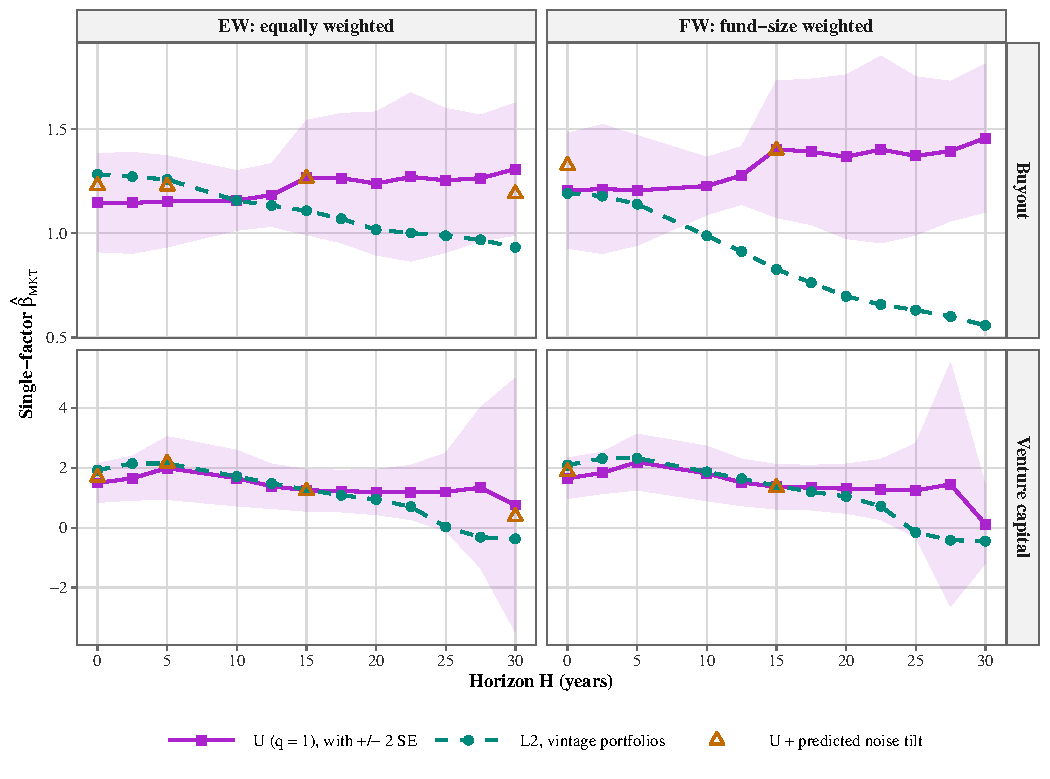
\includegraphics[width=0.85\textwidth]{figure_E1_beta_profiles.pdf}
\caption{Single-factor $\hat\beta_{MKT}$ across horizons: $U_{v,H}$ and L2}
\label{fig:u_beta_profiles}
\par\vspace{2pt}
{\scriptsize\textit{Notes:} North America, vintages up to 2010 (FW baseline: within-vintage median fund-size imputation; sensitivity in Table~\ref{tab:fw_imputation_sensitivity}): Buyout 25 vintages; VC 27, of which the 23 with at least two funds enter $U_{v,H}$. $U_{v,H}$: the cross-fund pair-product criterion with equal vintage weights ($q_v=1$); under Theorem~T7 (conditional independence of funds given the factor path, eligibility $n_v\ge2$, fund sizes, and vintage origin, zero conditional mean pricing error, no shared vintage effects $c_v=0$, and unique identification), it targets $\theta_0$ at every horizon, $H=0$ included. L2: squared loss on vintage portfolios (DLP12 at $H=0$), whose target is tilted by within-vintage fund noise and moves with $H$ (matched-vintage 23-vintage VC L2 reported in Table~\ref{tab:iv_comparison}). SE: Bartlett sandwich over vintage years, $S=\lceil1.3\sqrt V\rceil$. Shaded band: pointwise 95\% fixed-$b$ confidence band around $U_{v,H}$ ($\pm2.790$ SE for Buyout, $b=0.280$; $\pm2.867$ SE for VC, $b=0.304$), matching the table inference. Triangles: $U_{v,H}$ plus the expected estimator gap (mean L2 minus $U_{v,H}$, combining target shift and finite-sample difference) in the data-shaped core Monte Carlo without vintage-level effects (EW at 0, 5, 15 and 30 years; FW, with the data's fund-size dispersion, at 0 and 15 years). In VC, full-sample L2 uses 27 vintages while $U_{v,H}$ uses the 23 vintages with $n_v\ge2$; matched-vintage 23-vintage L2 gaps are reported alongside full-sample gaps in Table~\ref{tab:iv_comparison}. The headline estimate is $U_{v,H}$ at $H=0$; the profile across $H$ is a display, not a choice of horizon. Values: Tables~\ref{tab:u_l2_beta} and~\ref{tab:u_l2_beta_all}.}
\end{figure}
